\chapter{Procedimento Metodológico}
\label{Metodologia}

Este Capítulo detalha o processo metodológico para aprimorar a análise de ecocardiogramas, com foco na melhoria da precisão e eficiência das técnicas de análise de imagens médicas para calcular a fração de ejeção cardíaca. Iniciamos com a revisão sistemática da literatura na Seção \ref{Revisão Sistemática da Literatura} e a avaliação de trabalhos relevantes na Seção \ref{Avaliação de trabalhos potenciais}. Neste Capítulo, a Seção \ref{subsec:descricao_experimentos} descreve os experimentos realizados, enquanto a Seção \ref{Base de dados} aborda a seleção, aquisição e preparação dos conjuntos de dados essenciais. Na Seção \ref{Implementação da arquitetura modificada}, explicamos a implementação de uma arquitetura modificada, seguida pela nova combinação de parâmetros da rede neural na Seção \ref{Otimização de parâmetros}. Por fim, a Seção \ref{sub:Implementação} apresenta as tecnologias utilizadas na execução dos experimentos. A Figura \ref{fig:procedimento_metodologico} ilustra o fluxograma do processo metodológico adotado, abrangendo desde a revisão da literatura até a modificação dos parâmetros da rede neural.

\begin{figure}
    \centering
    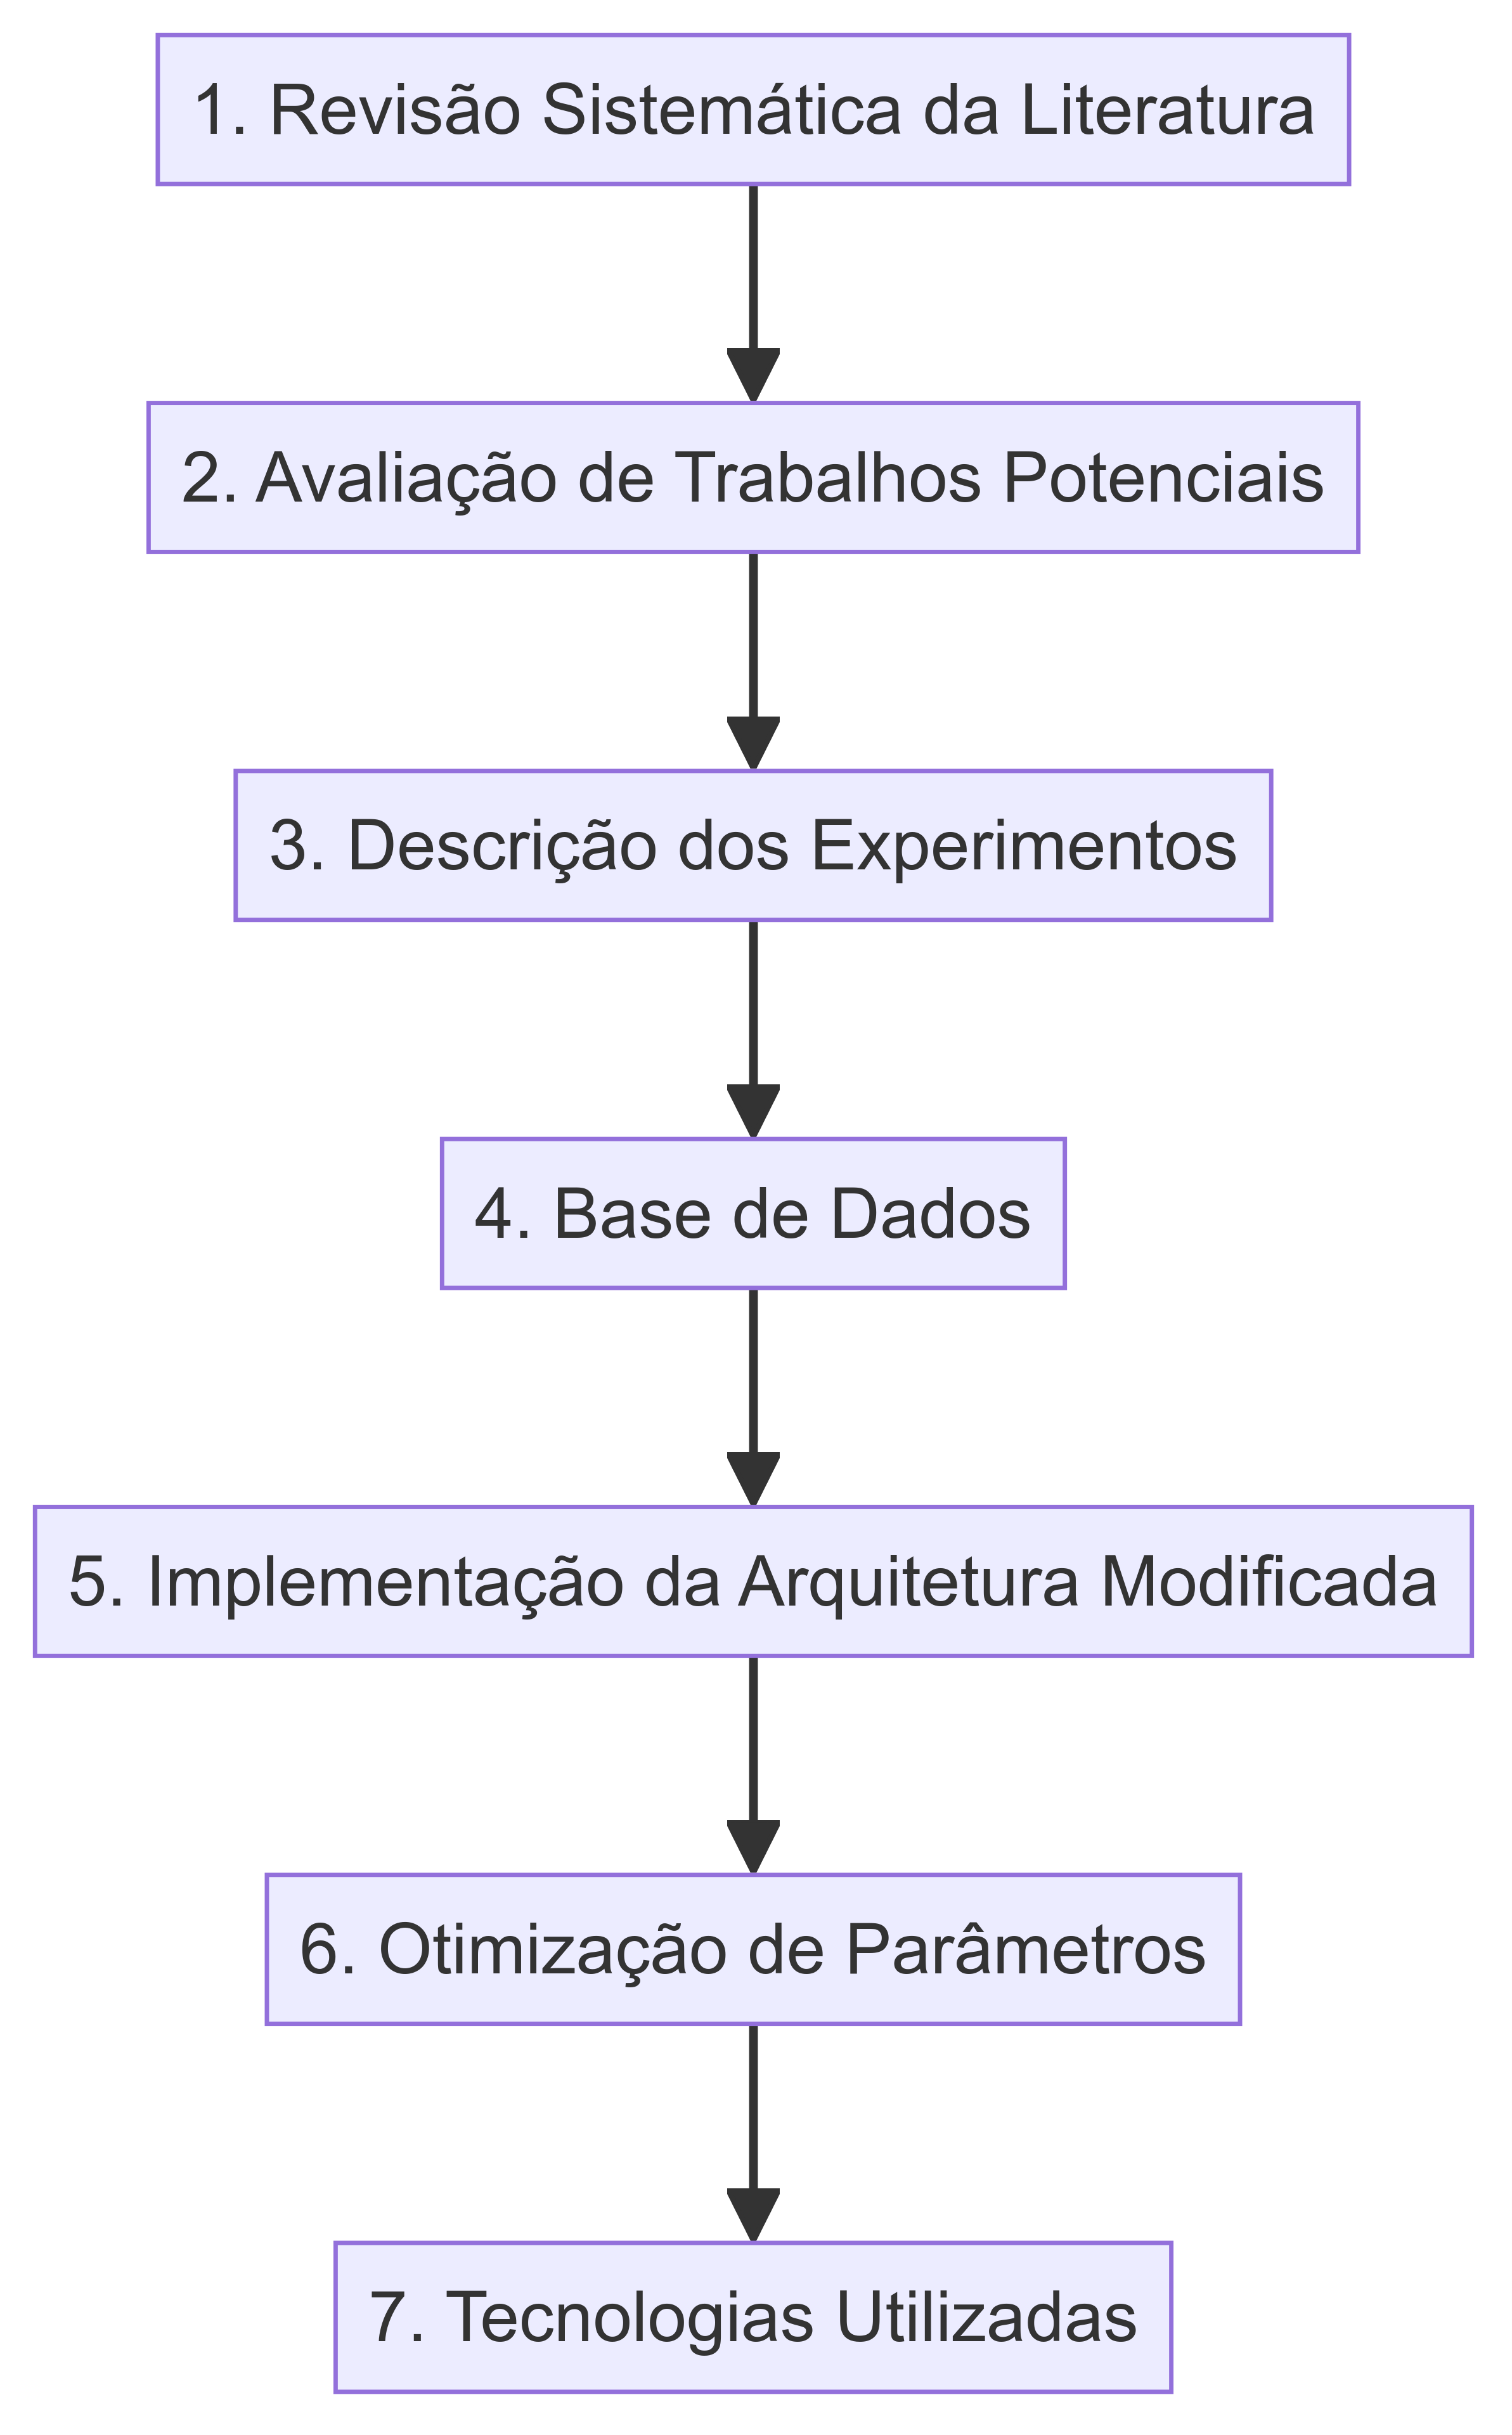
\includegraphics[width=0.5\linewidth]{capitulos//figuras/procedimentometo.png}
    \caption{Fluxograma do processo metodológico para análise de ecocardiogramas visando a melhoria da precisão e eficiência na determinação da fração de ejeção cardíaca.}
    \label{fig:procedimento_metodologico}
\end{figure}


\section{Descrição dos experimentos e justificativa}
\label{subsec:descricao_experimentos}

Foram realizados dois experimentos para avaliar a eficácia da arquitetura UViT e suas adaptações com diferentes bases de dados. O primeiro experimento utilizou a arquitetura UViT exatamente como desenvolvida por \textcite{Reynald} e descrita na Seção \ref{subsec:Redes neurais transformers}, juntamente com os conjuntos de dados do Echonet descritos na Seção \ref{Base de dados}. Este passo inicial é fundamental para estabelecer um ponto de referência comparativo (baseline), permitindo-nos avaliar posteriormente as vantagens e aprimoramentos introduzidos pelas metodologias subsequentes. Em seguida, avançamos para um segundo experimento, que envolve a versão adaptada da arquitetura UViT, que sera detalhada na Seção  \ref{Implementação da arquitetura modificada} e e nova combinação de parâmetros da rede neural na Seção \ref{Otimização de parâmetros}. Esta adaptação foi  aplicada aos conjuntos de dados Echonet e Echoped treinados de formas separadas e um experimento treinado de forma conjunta a fim de validar a hipótese de generalização dos dados. A comparação direta entre a arquitetura UViT clássica e sua versão modificada permite não apenas avaliar o impacto das alterações propostas, mas também destacar as melhorias específicas para dados pediátricos.

A escolha desses dois experimentos foi estratégica para permitir uma análise comparativa efetiva, fundamentando a importância das modificações na arquitetura UViT frente ao método original. A inclusão de dados pediátricos e a comparação dos resultados obtidos fornecem uma base para validar as vantagens das inovações implementadas, oferecendo uma contribuição significativa à precisão da estimativa da fração de ejeção em um contexto ampliado.

\section{Base de dados}
\label{Base de dados}

A escolha das bases de dados \textit{EchoNet-Dynamic} disponibilizado por \cite{Ouyang2020} e \textit{EchoNet Pediátricos} disponibilizado por \cite{Reddy2023} evidencia a intenção de incluir tanto a população adulta quanto a pediátrica, o que resulta em uma significativa extensão do alcance potencial da arquitetura UViT modificada.

A base de dados da  EchoNet-Dynamic contém 10.030 vídeos de ecocardiogramas apicais de 4 câmaras, coletados entre 2016 e 2018 no Hospital da Universidade de Stanford. Cada vídeo disponibilizado foi preparado, removendo textos e informações irrelevantes e padronizado para um formato de 112x112 pixels. Esta padronização é crucial para garantir a consistência e a qualidade dos dados para análises computacionais. Além dos vídeos, a EchoNet-Dynamic oferece medições clínicas e cálculos realizados por sonografistas registrados e verificados por um ecocardiografista de nível 3. Um dos principais indicadores clínicos presentes na base de dados é a fração de ejeção do ventrículo esquerdo, um parâmetro chave para o diagnóstico de cardiomiopatias, avaliação da elegibilidade para certas quimioterapias e determinação da necessidade de dispositivos médicos. Esta métrica é expressa como uma porcentagem, calculada pela razão do volume sistólico final  e o volume diastólico final do ventrículo esquerdo. A base de dados  também inclui traçados do ventrículo esquerdo, realizados no limite endocardíaco em dois momentos distintos: no final da sístole e no final da diástole. Estes traçados são utilizados para estimar o volume ventricular, integrando a área do ventrículo ao longo do eixo maior. Os traçados dos especialistas são representados por um conjunto de coordenadas emparelhadas, correspondentes a cada traçado humano. Estas coordenadas ajudam a determinar a orientação e o tamanho dos eixos do ventrículo esquerdo. A base de dados se encontra disponível em https://echonet.github.io/dynamic/. Acesso em: 03, Agosto de 2023.

A Echoped foi desenvolvido focando exclusivamente em dados pediátricos. Este conjunto de dados compreende 7.643 vídeos de ecocardiografia, cobrindo uma ampla gama de condições típicas de aquisição de imagens em laboratórios de ecocardiografia. Além de incluir medições como a fração de ejeção e volumes do ventrículo esquerdo no final da sístole e diástole. Os vídeos de ecocardiograma do conjunto de dados incluem imagens apicais de 4 câmaras e vistas do eixo curto parasternal, provenientes de pacientes atendidos no Lucile Packard Children’s Hospital em Stanford entre 2014 e 2021. Cada vídeo passou por um processo de edição para garantir a remoção de informações irrelevantes e padronização para o formato de 112x112 pixels, visando a consistência necessária para análises de alta qualidade.As medições clínicas vinculadas a cada vídeo, obtidas e verificadas por especialistas, adicionam um valor inestimável ao conjunto de dados. A métrica da fração de ejeção do ventrículo esquerdo. Além disso, os traçados especializados do ventrículo esquerdo, em momentos específicos do ciclo cardíaco, fornecem dados precisos para estimativas de volume ventricular. A base de dados se encontra disponível em https://echonet.github.io/pediatric/. Acesso em: 28, julho de 2023.


\section{Implementação da arquitetura modificada}
\label{Implementação da arquitetura modificada}

Nessa Seção descrevemos a elaboração e aprimoramento do pipeline para análise de imagens de ecocardiograma, iniciando com a arquitetura base UViT, conforme descrito por \textcite{Reynald}. O primeiro elemento deste pipeline foi projetado para enfrentar os desafios computacionais associados ao processamento de imagens completas de ultrassom, especialmente em formatos de vídeo. Esta etapa foca na manipulação eficiente dos frames de vídeo, que são as imagens individuais sequenciadas para formar o vídeo completo. Adotamos uma estratégia de redução de dimensionalidade, utilizando a Seção de codificação de uma Arquitetura de Autoencoder Residual (ResNetAE), como ilustrado na Figura \ref{fig:resnetAE}. Esta abordagem converte os frames em representações vetoriais compactas, reduzindo significativamente a carga computacional na análise direta das imagens.

A manutenção dessa abordagem específica é crucial, caracterizando-se pela incorporação de blocos residuais em múltiplas escalas tanto no codificador quanto no decodificador. Essa configuração permite uma agregação eficiente de informações através das dimensões espaciais das imagens, facilitando a captura de características relevantes em diferentes níveis de granularidade. Esta estratégia revela-se particularmente vantajosa para a análise complexa de imagens de ultrassom. Além disso, a otimização de hiperparâmetros, que inclui ajustes na profundidade do codificador e no tamanho do espaço latente, é crítica para a configuração da arquitetura do Autoencoder. Este processo de otimização, realizado através de uma tarefa de reconstrução especificamente adaptada ao conjunto de dados de ultrassom, assegura que a arquitetura esteja finalmente sintonizada com as características únicas desses dados, maximizando assim o desempenho e a precisão do modelo.

Prosseguindo nesta direção, a configuração ótima do codificador, resultante deste processo de otimização, é reintegrada ao pipeline como o componente essencial de codificação. Assim, cada quadro é processado pelo codificador transformando-se em um vetor de 1024 dimensões. As representações vetoriais resultantes são organizadas para formar a representação vetorial inicial do clipe, estruturado em uma matriz Batch (lote de dados, representando a quantidade de exemplos de treinamento processados em conjunto) × Nframes (número de quadros, indicando a quantidade de imagens ou frames de vídeo no clipe) × 1024. Esta etapa, importante para a preparação dos dados para análise subsequente, mantém-se inalterada em relação à estratégia original, preservando a abordagem estabelecida para a redução de dimensionalidade.


\begin{figure}
    \centering
    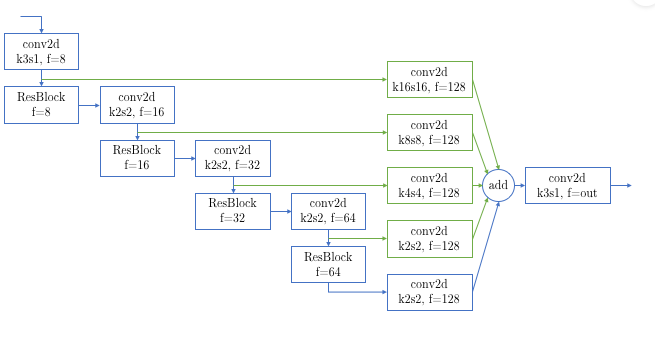
\includegraphics[width=1\linewidth]{image.png}
   \caption{Arquitetura ResNetAE de \textcite{ResNetAE} }
    \label{fig:resnetAE}
\end{figure}

No desenvolvimento do segundo módulo da arquitetura Ultrassom Video Transformer (UViT), houve uma significativa incorporação de tecnologias provenientes do processamento de linguagem natural (PLN), mais notavelmente RoBERTa (Robustly optimized BERT approach). Estes avanços metodológicos são fundamentais para a análise de conteúdo visual e são particularmente eficazes no tratamento de vídeos de ultrassom, promovendo uma compreensão espaço-temporal aprimorada.

RoBERTa, que evolui a partir do BERT (Bidirectional Encoder Representations from Transformers), se sobressai por sua extensiva capacidade de treinamento em vastos conjuntos de dados e um número incrementado de iterações, o que resulta em uma análise mais detalhada dos aspectos espaço-temporais dos vídeos. Uma mudança crítica na transição do BERT para o RoBERTa é a remoção do objetivo de Previsão de Próxima Sentença (NSP), o que foi demonstrado por \textcite{Roberta} manter ou até mesmo aprimorar o desempenho em diversas tarefas de PLN. O RoBERTa também se beneficia do uso de lotes de dados maiores e sequências mais extensas durante o treinamento, o que diverge do protocolo original do BERT e contribui para um avanço na modelagem de linguagem mascarada e na precisão de tarefas específicas de linguagem natural.

A escolha de RoBERTa para a arquitetura UViT permite uma análise mais profunda e detalhada, maximizando a eficácia na interpretação de vídeos de ecocardiograma. Tal mudança não apenas eleva o padrão de análise espaço-temporal para vídeos de ultrassom, mas também estabelece um novo paradigma para a aplicação de técnicas de PLN na análise visual, evidenciando o potencial transformador de adaptar e combinar metodologias de inteligência artificial novas como as redes transformers.

Para conduzir análises espaço-temporais em vídeos de durações variáveis, utilizamos um modelo de Reconhecimento de Entidades Nomeadas (\textit{NER}) baseado em vídeo. Este modelo emprega incorporações vetoriais derivadas de uma etapa de codificação com o uso de ResNetAE (\textit{Autoencoder Residual}) de \textcite{ResNetAE}, que codifica as características visuais essenciais do vídeo. As incorporações vetoriais resultantes são fundamentais e são processadas pelos codificadores RoBERTa. A função de cada codificador, indexada por \(k\), é matematicamente representada pela Equação \ref{eq:encoder_function}.

\begin{equation}
B_k(E) = \text{LayerNorm}\left(D_{k,c}\left(\text{GELU}\left(D_{k,b}\left(A_k(E)\right)\right)\right) + S_k(E)\right),
\label{eq:encoder_function}
\end{equation}

No contexto das redes Transformer, \(S_k(E)\) denota o bloco de Autoatenção, que é responsável por calcular os pesos de atenção normalizados. Esses pesos são derivados do produto escalar entre as matrizes de Consulta (\(Q_k(E)\)) e Chave (\(K_k(E)\)), ajustados por um fator de escala. Este fator é dependente da relação entre a dimensionalidade das incorporações vetoriais (\(n_d\)) e o número de cabeças de atenção (\(n_B\)). A equação correspondente é apresentada em \ref{eq:self_attention}. Uma explicação mais detalhada sobre redes Transformer e seus componentes é fornecida na Seção \ref{subsec:Redes neurais transformers}.



\begin{equation}
S_k(E) = \text{Softmax}\left(\frac{Q_k(E)K_k^T(E)}{\sqrt{\frac{n_d}{n_B}}}\right)V_k(E),
\label{eq:self_attention}
\end{equation}


E \(A_k(E)\) indica o bloco de Atenção, integrando as saídas de \(S_k(E)\) com as incorporações vetoriais originais \(E\), seguido por uma camada de normalização, também conhecida como Layer Normalization, é uma etapa crítica no processamento dos incorporações vetoriais e é dada pela Equação \ref{eq:attention_integration}.

\begin{equation}
A_k(E) = \text{LayerNorm}\left(D_{k,a}\left(S_k(E)\right) + E\right).
\label{eq:attention_integration}
\end{equation}

Neste cenário avançado, as matrizes \( Q _k \), \( K_k \), e \( V_k \) atuam como transformações lineares essenciais, designadas respectivamente às funções de Consulta (Query), Chave (Key) e Valor (Value), fundamentais na arquitetura de autoatenção. Estas matrizes são responsáveis por converter os dados de entrada em representações mais significativas que facilitam a identificação de padrões relevantes para a tarefa em questão. As camadas \( D_{k,\{a,b,c\}} \)  representam camadas densas intermediárias que exercem uma função crítica na reformulação dos dados processados pelo codificador, permitindo uma manipulação mais refinada das informações. Os parâmetros ajustáveis \( n_B \) e \( n_D \) referentes ao tamanho do batch e à dimensão dos embeddings, respectivamente, são  calibrados para encontrar um equilíbrio ótimo entre a capacidade de processamento e a eficiência computacional. Este ajuste fino visa aprimorar o desempenho do modelo na análise de vídeos de ecocardiograma, garantindo que o sistema seja capaz de processar informações complexas de forma eficaz, sem comprometer a rapidez e a precisão das previsões. A otimização desses parâmetros é um processo iterativo que envolve a experimentação e a validação cruzada para assegurar que o modelo esteja ajustado para oferecer a melhor performance possível.

No terceiro componente do nosso pipeline de análise de vídeos, a integração das saídas dos $k$ codificadores, seja eles para o RoBERTa do módulo anterior, denotadas por $B_k(E)$, com a saída do ResNetAE, $E$, é realizada por meio de uma média ponderada. Esta abordagem visa combinar  as representações espaço-temporais capturadas pelos codificadores RoBERTa com as características espaciais codificadas pelo ResNetAE. A formulação matemática para a matriz de características composta $M(E)$ é dada pela Equação \ref{eq:equacao_norm}.


\begin{equation}
M(E) = \frac{1}{n_B + 1} \left( E + \sum_{k=1}^{n_B} B_k(E) \right),
\label{eq:equacao_norm}
\end{equation}

onde:
\begin{itemize}
    \item $E$ representa as incorporações vetoriais obtidas pela aplicação do ResNetAE sobre as imagens de ultrassom, funcionando como a base para características espaciais.
    \item $B_k(E)$ é a matriz de saída do $k$-ésimo codificador, seja RoBERTa, que foi aplicado para potencializar $E$ com informações espaço-temporais. Esta matriz contém vetores de embedding para cada elemento processado, com cada vetor representando a informação espaço-temporal enriquecida de um único frame ou segmento de vídeo. A dimensão da matriz reflete o número de elementos processados e a dimensão dos embeddings gerados pelo codificador.
    \item $n_B$ indica o número total de codificadores RoBERTa empregados, possibilitando uma análise detalhada e diversificada através da combinação de múltiplas representações espaço-temporais.
    \item $M(E)$ é a matriz de características composta, que integra as dimensões espaciais e espaço-temporais em uma única representação. Esta matriz é o resultado da combinação ponderada de $E$ com as saídas $B_k(E)$ de todos os codificadores utilizados, fornecendo uma base rica e multifacetada para a fase de regressão subsequente.
\end{itemize}


A eficácia desta abordagem combinatória origina-se da integração de duas dimensões essenciais na análise de imagens de ultrassom. Primeiramente, exploramos a dimensão espacial, que envolve a análise da estrutura e anatomia visíveis nas imagens. Utilizando o ResNetAE, não só reduzimos a dimensionalidade das imagens para facilitar o processamento subsequente, mas também extraímos características físicas, como por exemplo a forma do coração e a textura dos tecidos. Esta análise é fundamental para entender a condição estrutural do órgão. Em seguida, adicionamos a dimensão espaço-temporal, que capta as variações e movimentos ao longo do tempo, essenciais para analisar os ciclos cardíacos. Essa dimensão é reforçada pelos codificadores RoBERTa, que analisam a sequência dos quadros para detectar padrões de movimento, como expansão e contração durante a sístole e diástole.

Essas duas dimensões são então integradas em uma única matriz de características, denominada \(M(E)\). Esta matriz representa um conjunto compacto e integrado de dados que combina informações espaciais e espaço-temporais. O processo envolve a agregação de vetores de características extraídos de cada quadro de vídeo, resultando em uma representação unificada que potencializa a análise e a precisão dos modelos de regressão. A precisão aprimorada obtida com \(M(E)\) é crucial para identificar com exatidão os momentos específicos dos ciclos cardíacos, como os pontos de início e fim da sístole e diástole, além de calcular a fração de ejeção.


Essa matriz \(M(E)\) é submetida a dois regressores: um destinado a prever os índices de início da sístole (ES) e diástole (ED) mostrado na figura \ref{fig:reg01}, \(R_{SD}(M(E))\), e outro para calcular a Fração de Ejeção do Ventrículo Esquerdo mostrado na Figura \ref{fig:fraceject} , \(R_{EF}(M(E))\). O regressor \(R_{SD}\) é formulado como a saída de três camadas lineares intercaladas com normalização por camadas, finalizando com uma ativação tangente hiperbólica (tanh). A função tanh é escolhida por sua eficácia em normalizar a saída do modelo para um intervalo entre -1 e 1, facilitando a estabilização do treinamento e a interpretação dos resultados finais. A fração de ejeção do ventrículo esquerdo é expressa pela Equação \ref{eq:01}, com \(n_F\) representando o número de quadros de entrada. A rede de regressão reduz a dimensão das incorporações vetoriais para 1 para cada quadro de entrada, e a média dessas previsões individuais produz uma única estimativa de fração de ejeção do ventrículo esquerdo por vídeo. Este processo de redução de dimensões é importante, pois transforma dados complexos e de alta dimensionalidade em uma forma mais tratável que enfatiza as características mais relevantes para a tarefa de predição, maximizando a eficiência computacional e a precisão do modelo.


\begin{equation}
R_{EF}(M(E)) = \text{Sigmoid} \left( \frac{1}{n_F} \sum_{f=1}^{n_F} D_{EF,2} \left( \text{LayerNorm} \left( D_{EF,1} (M(E)) \right) \right) \right)
\label{eq:01}
\end{equation}



\begin{figure}
    \centering
    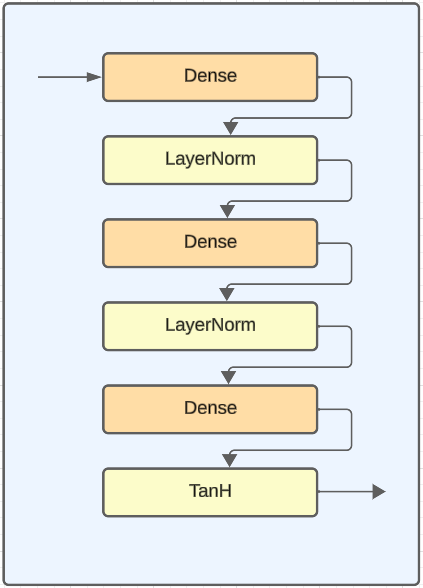
\includegraphics[width=0.5\linewidth]{imagereg.png}
    \caption{Ramo de regressão sistole-diástole}
    \label{fig:reg01}
\end{figure}



\begin{figure}
    \centering
    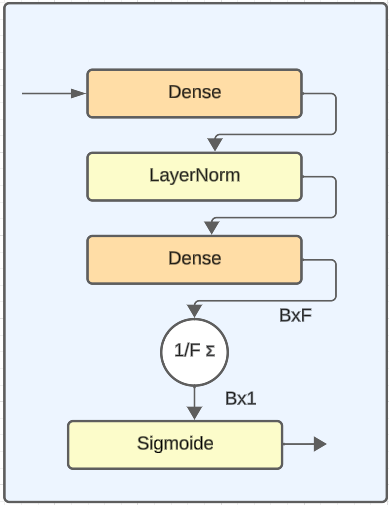
\includegraphics[width=0.5\linewidth]{reg02.png}
    \caption{Ramo de regressão para calculo da fração de ejeção}
    \label{fig:fraceject}
\end{figure}


Para otimizar a precisão na previsão da Fração de Ejeção do Ventrículo Esquerdo, adotamos uma abordagem de treinamento que integra tanto a minimização de erros quanto a aplicação de \textit{regularização}, visando corrigir desequilíbrios na distribuição de fração de ejeção do ventrículo esquerdo no conjunto de dados. As métricas de erro empregadas são o \textit{Mean Squared Error} (\textit{MSE}) e o \textit{Mean Absolute Error} (\textit{MAE}), definidos respectivamente pelas Equações \ref{eq:MSE} e \ref{eq:MAE}.

\begin{equation}
L_{\text{MSE}}(\hat{y}, y) = \frac{1}{n_F} \sum_{f=1}^{n_F} (\hat{y}_f - y_f)^2,
\label{eq:MSE}
\end{equation}

Na Equação \ref{eq:MSE}, \(L_{\text{MSE}}(\hat{y}, y)\) é a função de perda MSE, onde \(\hat{y}\) é o valor previsto, \(y\) é o valor real, e \(n_F\) é o número total de quadros de entrada. A função de perda MSE calcula a média dos quadrados das diferenças entre os valores previstos e reais.

\begin{equation}
L_{\text{MAE}} = \frac{1}{n_F} \sum_{f=1}^{n_F} \left| \hat{y}_f - y_f \right|,
\label{eq:MAE}
\end{equation}

Na Equação \ref{eq:MAE}, \(L_{\text{MAE}}\) é a função de perda MAE, onde \(\hat{y}\) é o valor previsto, \(y\) é o valor real, e \(n_F\) é o número total de quadros de entrada. A função de perda MAE calcula a média das diferenças absolutas entre os valores previstos e reais.


A fim de enfatizar o treinamento na estimativa da fração de ejeção do ventrículo esquerdo e mitigar desvios significativos das previsões em relação a um valor de referência $\gamma$ — aproximadamente a média da fração de ejeção do ventrículo esquerdo no conjunto de treinamento —, introduzimos um termo de regularização $R(y)$, conforme a Equação \ref{eq:Reg}.

\begin{equation}
R(y) = (1 - \alpha) + \alpha \cdot \frac{\lVert y - \gamma \rVert}{\gamma},
\label{eq:Reg}
\end{equation}

O parâmetro $\alpha$ calibra a intensidade da penalidade para estimativas de Fração de Ejeção do Ventrículo Esquerdo (FEVE) que divergem do valor de referência $\gamma$, proporcionando uma sintonia refinada na penalização de desvios do alvo FEVE.

Assim, a função de custo total $L_{EF}$, que o modelo visa minimizar durante o processo de treinamento, é formulada pela combinação das métricas de erro ponderadas pelo termo de regularização, conforme expresso pela Equação \ref{eq:LEF}.


\begin{equation}
L_{EF} = (L_{MSE} + L_{MAE}) \cdot R(y).
\label{eq:LEF}
\end{equation}

Esta formulação assegura que, além de aprender a reduzir os erros de previsão diretamente, o modelo ajusta suas estimativas para alinhar-se mais estreitamente com a distribuição esperada de fração de ejeção do ventrículo esquerdo no conjunto de treinamento, abordando assim os desafios impostos por possíveis desequilíbrios na distribuição das fração de ejeção do ventrículo esquerdo.

\section{Nova combinação de hiperparâmetros}
\label{Otimização de parâmetros}

Essa Seção busca aprimorar o desempenho do novo modelo em comparação ao descrito por \textcite{Reynald}. Uma reconfiguração dos hiperparâmetros foi executada. Assim, ampliamos o \textit{Attention Head} de 16 para 32, o que amplia a capacidade do modelo de processar informações em paralelo, melhorando significativamente a atenção aos detalhes sutis nos dados e reforçando a capacidade de generalização. 

Além disso, o incremento do \textit{Number of Hidden Layers} de 16 para 32 permite ao modelo captar e representar hierarquias mais sofisticadas de características, essenciais para a compreensão aprofundada de contextos e relações complexas nos dados. Essa representação aprimorada é um fator determinante para o aumento da precisão das previsões.

A duplicação do \textit{Batch Size} contribui não apenas para a eficiência computacional, permitindo que o modelo processe mais dados em simultâneo e acelere o treinamento, mas também promove uma estimativa do gradiente mais robusta, ajudando a mitigar o risco de \textit{overfitting}.

Para otimizar a utilização dos recursos de memória da GPU, o \textit{Max Length (dsmax)} foi reduzido de 128 para 64, prevenindo a exaustão da memória e garantindo a eficácia do treinamento. Este ajuste é uma medida preventiva que assegura a operacionalidade do modelo dentro das limitações de hardware, mantendo a qualidade do treinamento apesar do aumento das demandas computacionais devido às camadas adicionais e ao tamanho do lote expandido.
Esta etapa busca aprimorar o desempenho do novo modelo em comparação ao descrito por \textcite{Reynald}. Uma reconfiguração dos hiperparâmetros foi executada. Assim, ampliamos o \textit{Attention Head} de 16 para 32, o que amplia a capacidade do modelo de processar informações em paralelo, melhorando significativamente a atenção aos detalhes sutis nos dados e reforçando a capacidade de generalização.

Além disso, o incremento do \textit{Number of Hidden Layers} de 16 para 32 permite ao modelo captar e representar hierarquias mais sofisticadas de características, essenciais para a compreensão aprofundada de contextos e relações complexas nos dados. Essa representação aprimorada é um fator determinante para o aumento da precisão das previsões.

A duplicação do \textit{Batch Size} contribui não apenas para a eficiência computacional, permitindo que o modelo processe mais dados em simultâneo e acelere o treinamento, mas também promove uma estimativa do gradiente mais robusta, ajudando a mitigar o risco de \textit{overfitting}.

Para otimizar a utilização dos recursos de memória da GPU, o \textit{Max Length (dsmax)} foi reduzido de 128 para 64, prevenindo a exaustão da memória e garantindo a eficácia do treinamento. Este ajuste é uma medida preventiva que assegura a operacionalidade do modelo dentro das limitações de hardware, mantendo a qualidade do treinamento apesar do aumento das demandas computacionais devido às camadas adicionais e ao tamanho do lote expandido.

Os seguintes parâmetros não foram modificados, com as seguintes justificativas: A *taxa de aprendizado (learning rate, lr)* foi mantida em \(1 \times 10^{-5}\) (a velocidade com que o modelo aprende com os dados durante o treinamento). Essa taxa é escolhida para garantir um aprendizado controlado e estável, minimizando oscilações bruscas durante o treinamento que poderiam prejudicar a convergência do modelo. A *dimensão latente (latent\_dim)* continua em 1024 (o tamanho do vetor que representa as características aprendidas dos dados). Identificamos que uma alteração nesse parâmetro não traria benefícios adicionais, uma vez que essa configuração já provou ser suficiente para capturar as características essenciais dos dados, e aumentá-la resultaria em um modelo muito grande, incapaz de ser processado na GPU disponível, sem trazer os benefícios esperados. O *período de passo da taxa de aprendizado (lr\_step\_period)* é mantido em 3 épocas (a frequência com que a taxa de aprendizado é ajustada para garantir eficiência), que é o intervalo antes da taxa de aprendizado ser dividida por 10. Esse procedimento permite uma redução gradual e controlada da taxa, facilitando uma convergência mais estável e eficiente do modelo. Finalmente, o *espaçamento mínimo entre quadros (ds\_min\_spacing)* foi mantido em 10 quadros (o número mínimo de quadros entre amostras durante o treinamento) para assegurar que a densidade dos quadros processados seja adequada, evitando sobrecarga de processamento e garantindo uma boa representação temporal dos dados. Essas decisões visam otimizar o processo de treinamento, mantendo a eficácia e a eficiência do modelo.

Todas essas modificações foram implementadas com a premissa de que um modelo com maior capacidade e eficiência computacional pode aprender representações mais complexas e abstratas dos dados


\section{Implementação} 
\label{sub:Implementação}

Na quinta etapa do projeto, foi estabelecido um ambiente de desenvolvimento utilizando \textit{Docker}, garantindo isolamento e reprodutibilidade nas execuções da implementação e testes. Esse ambiente operou com a linguagem \textit{Python} e utilizou as bibliotecas \href{https://pytorch.org/}{\textit{PyTorch}} e \href{https://huggingface.co/transformers/}{\textit{transformers}}, que são reconhecidas por sua ampla funcionalidade em projetos de aprendizado de máquina e inteligência artificial. A estrutura de processamento paralelo foi implementada utilizando oito placas de GPU \textit{Tesla Pascal} (modelo P100-SXM2-16GB), cada uma equipada com 16GB de memória e 3584 \textit{cores CUDA}, totalizando 28672 \textit{cores CUDA}. Esse \textit{setup} permitiu uma execução paralela eficaz, sendo crucial para o processamento de grandes volumes de dados e análise computacional intensiva.

Para suportar as elevadas demandas de processamento, a máquina escolhida para este ambiente estava equipada com dois processadores \textit{Intel Xeon E5-2698 v4}, cada um com 20 cores e 40 \textit{threads}, somando um total de 40 cores físicas e 80 \textit{threads} lógicas. Além disso, a máquina foi configurada com 512 GB de RAM e um armazenamento em \textit{SSD} de 7TB, proporcionando uma capacidade adequada para a manipulação eficiente de dados e execução de operações que requerem intensa utilização de memória.

O modelo desenvolvido está disponível em \url{https://github.com/thiago092/UVIT_MODIFICADO/}

